% Chapter 4

\chapter{Approach}

\label{approach}
The following sections will deeply explore and describe the insights of the project and the development process and the decisions taken with the reasons behind it. 
These sections imply a higher technical language and background filled with several domain-specific vocabularies.

%----------------------------------------------------------------------------------------

\section{Environment Architecture}
In this section, the different methodologies, programming tools and abstractions used during the project may be discussed and how the code is built around them.

\subsection{Python}
Python is a multi-purpose open-source programming language focused on the quick prototyping. Using a really simple language syntax makes any inexperienced programmer be able to comprehend and create simple scripts. 
Since there is no compilation, the debugging step is especially fast and repeating the cycle of editing and running is reduced in time\cite{pythonabout}.
Given the multiple open-source libraries and frameworks available for Machine Learning and Artificial Intelligence, Python is a great and suitable option to develop a project with the needed characteristics.
Some of the mentioned libraries that will be used along with the project:

\begin{itemize}
    \item NumPy: package for scientific computing with Python \cite{numpy}.
    \item pandas: library providing high-performance, easy-to-use data structures, and data analysis tools for the Python programming language \cite{pandas}.
    \item scikit-learn: Machine Learning module providing efficient tools for data mining and data analysis \cite{scikit}.
    \item Matplotlib  2D plotting library \cite{matplotlib}.
    \item seaborn: data visualization library. It provides a high-level interface for drawing attractive and informative statistical graphics \cite{seaborn}.
\end{itemize}


\subsection{MongoDB}
MongoDB is a general-purpose, document-based, distributed database \cite{mongo}.
With a powerful query syntax and language is pretty straightforward to build complex databases and retrieve the desired records with ease.
Since it is based on the JSON\cite{json} standard it allows creating complex records using arrays, nested properties, and key-value pairs.
Despite the traditional relation Databases using the SQL standards, MongoDB is a nonrelational database relaying on the NoSQL (Not Only SQL) syntax and instead of using tables and rows as in relational databases, MongoDB is built around collections and documents.

Given the previously described problem, MongoDB is a perfect and suitable option to depend on for storing and retrieving the music datasets available. With just some simple commands it easy to obtain the desired data, a chunk of it or more complex subsets that need to fit special conditions to better approximate the model standards.

\subsection{Tensorflow}
Tensorflow is an open-source mathematical computing library used as a backend for heavily expensive operations.
It offers different levels of abstractions so it can work easily coupled with different libraries that rely on heavy calculations and operations with matrixes or tensors.

It provides a collection of workflows to develop and train models using different programming languages so even though it was publicly released in 2015 it is the preferred option to build Machine Learning models as Artificial Neural Networks, the main topic of this thesis \cite{tensorflow}.

\subsection{Keras}
Keras is a high-level neural networks API, capable of running on top of TensorFlow. 
It is focused on enabling fast experimentation and prototyping using a friendly user-interface API, modularity, and extensibility. 

Supports most of the most common known Artifical Neural Networks types such a Deep Neural Networks, Convolutional Neural Networks, and Recurrent Neural Networks or any combination of the previously mentioned ones. 
Nonetheless, implementing your custom layers and metrics is easy in case the basic framework does not suit your needs.

Relying on TensorFlow as the mathematical background allows running seamlessly on both the CPU and the GPU thus heavy models with extensive training phases can be easily computed across different machines alleviating the load from one system to multiple ones.

\newpage
%----------------------------------------------------------------------------------------

\section{Basic stack}
The following section briefly explains how the components already mentioned are connected and used during the whole project.
The project consists of several scripts that handle each one of the individual tasks, only the main ones will be discussed in this paper:

\begin{itemize}
    \item Database Warmer: This script takes the provided CSV files to process them and creates a ready-to-use document for each of the songs to be inserted into the MongoDB Database. This is a one-use-only script that is crucial to be able to retrieve the desired songs afterward.
    \begin{figure}[th]
        \centering
        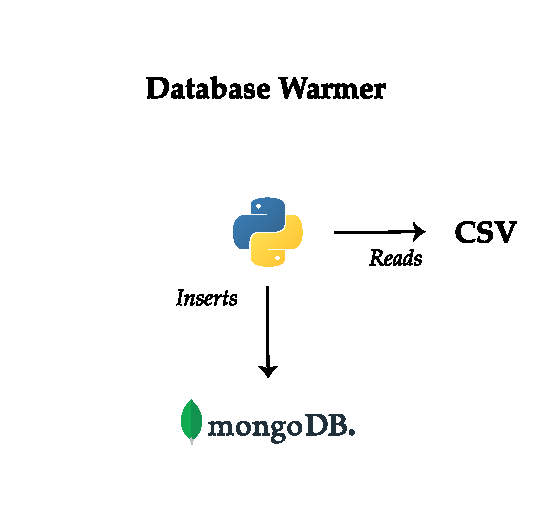
\includegraphics{Figures/DatabaseWarmer}
        \decoRule
        \caption[Database Warmer Script]{Diagram detailing the database warming process}
        \label{fig:Database Warmer Script}
    \end{figure}


    Here is an example of one of the documents inserted:
    \begin{lstlisting}[caption=Song JSON document]
{
    "_id": "5cadfc2f4fac9e1e50b0ad5a",
    "mbid": "1a00a335-fead-46ec-8d4f-06e8341291ea",
    "release": "0f2ccf4d-d242-3c23-a419-ea548af51df3",
    "genres": [
        {
        "name": "electronic",
        "genres": [
            {
            "name": "ambient",
            "genres": []
            },
            {
            "name": "trance",
            "genres": []
            }
        ]
        }
    ]
}
    \end{lstlisting}

    
    \item Main Script This script is in charge of the entire process and stages model related:
    \begin{enumerate}
        
        \item Train: This is the base stage of the process, the script connects with the Database and retrieves the dataset to be used as training, loads and builds the model in Keras and proceeds to train the model using TensorFlow, once the training process is finished the trained model is stored in the disk and the results are evaluated in the test stage.
        \begin{figure}[th]
            \centering
            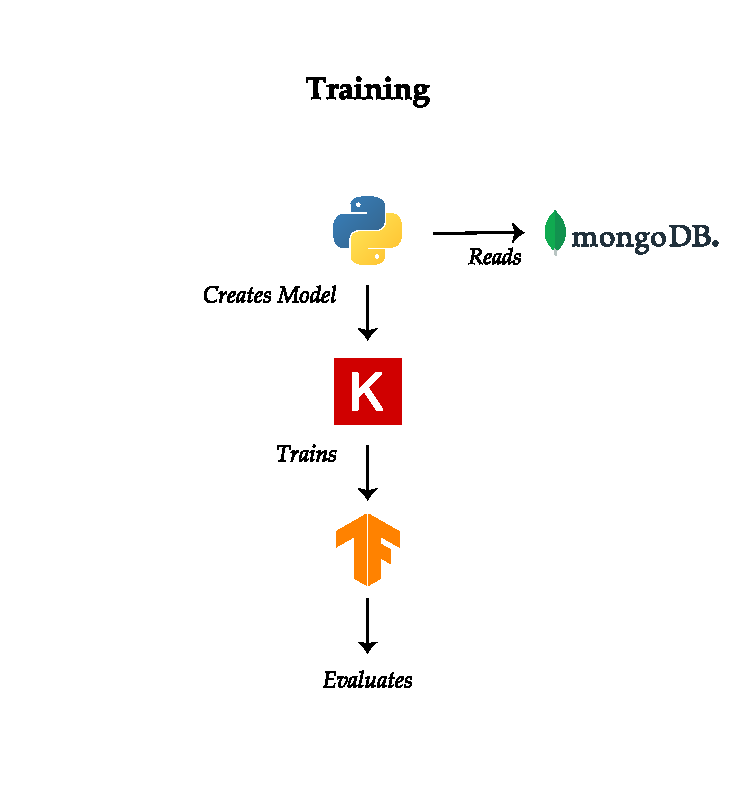
\includegraphics{Figures/TrainStage}
            \decoRule
            \caption[Train Stage]{Diagram detailing the training stage}
            \label{fig:Train Stage}
        \end{figure}
        
        \item Test: Once the model is trained its performance should be evaluated with data apart from the examples used in the training, to avoid the overfitting. For this case of the matter, the new examples are fed to the trained model and its outputs predicted and checked against its known outputs.
        \begin{figure}[th]
            \centering
            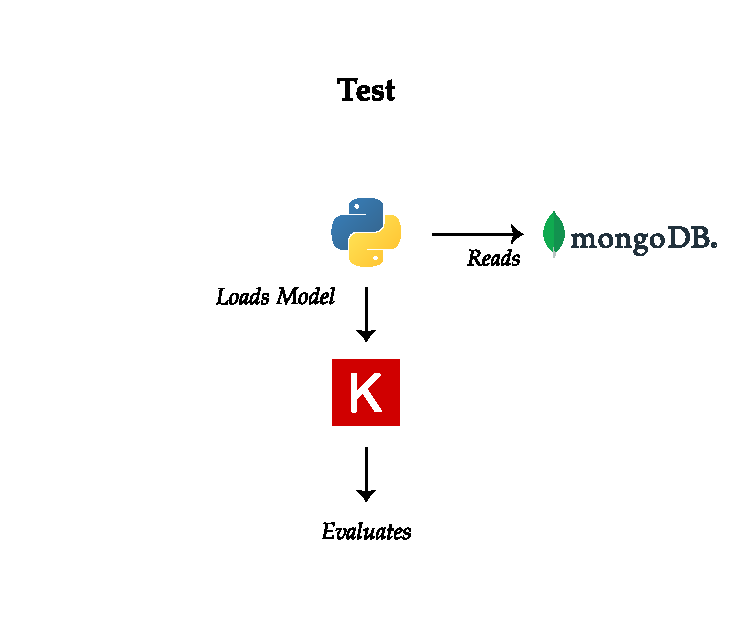
\includegraphics{Figures/TestStage}
            \decoRule
            \caption[Test Stage]{Diagram detailing the test stage}
            \label{fig:Test Stage}
        \end{figure}
        
        \item Predict: This phase is obtained once the proper model with the best outcome is built and trained. It properly labels new and unknown songs.
        \begin{figure}[th]
            \centering
            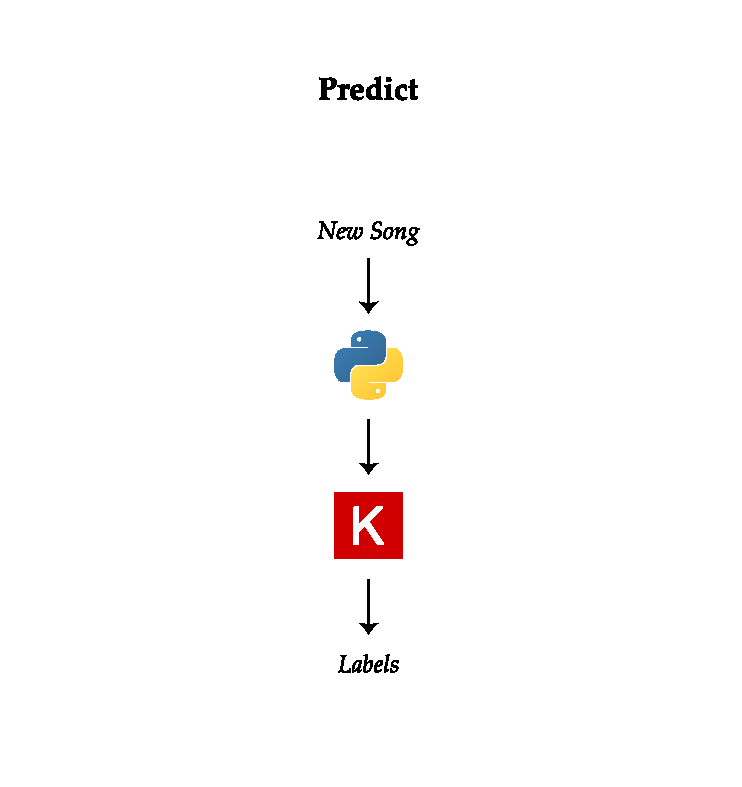
\includegraphics{Figures/PredictStage}
            \decoRule
            \caption[Predict stage]{Diagram detailing predict stage}
            \label{fig:Predict Stage}
        \end{figure}

    \end{enumerate}

\end{itemize}

\newpage
%----------------------------------------------------------------------------------------

\section{Initial approach}
\label{initialapproach}

In this section, the initial model and its next iterations will be discussed and explained along with the different design options taken during the process.

As mentioned in previous sections this thesis constitutes a Multi-Label classification problem,
so using the related work and state of art \ref{multilabelclassification} as a starting point there are two main architectures:

\subsection{Regular Multi Layer Perceptron (MLP)}
\label{approach MLP}

This method produces a single output for each of the songs fed and it has a neuron in the last layer for every genre $N$ available. Each one of those \(N\) neurons will hold the probability of that genre being present given an example \(x\) using the following expression:
$$ P(\hat{y} = i | x) \forall i \in N$$
This produces a probability vector $\hat{Y}$ that is pruned using a threshold value to obtain the highest probability genres.

The target $Y$ is obtained using the following mapping
$$
\bar{y_i} =
\begin{cases} 
    1 & \text{if } y_j \in S\\
    0 & \text{if } y_j \notin S\\
\end{cases}
\forall j \in N
$$

So given an example with the following genres:

$$ y  = [ Pop, Rock ]$$

And the available genres in the set:
$$ S  = [Jazz, Pop, Rock, Soul]$$
Will produce the output:
$$ \bar{y}  = [0, 1, 1, 0]$$

Then $Y$  is constructed as follows
$$ Y = [y_0, y_1, y_2 ... y_m]^T$$
Where $m$ is the number of examples to feed to the network.

To avoid overfitting it is important to provide a balanced dataset $Y$ otherwise the Network may suffer from overfitting.
To do so some artificial balancing methods such as SMOTE\cite{Chawla2002} \cite{Blagus2013} may be used

In general:
$$ |y^i| \approx \frac{m}{N}   \forall i \in N $$
being:
$$ m > N $$
And:
$$ \sum_{i=1}^{N} |y^i| \approx m $$

\subsection{Multi-label Multi-class Perceptron (MMP)}
\label{approach MMP}

This method differs from the previous one as several classifiers $c_i$ are trained for each of the available genres $N$. 
Each one of the classifiers will provide the statistical probability of a song being of that genre.
This creates an ensemble of classifiers $C$ :
$$ C = \{c_1, c_2, c_3 ... c_N\} $$ 

So given a predict function  $f(x, c)$, an example $x$ and a classifier $c_i$ 

$$ f(x, c_i) =  P(\hat{y_i} = i | x) \forall i \in N $$

Therefore the complete predicted vector $\hat{y}$ is defined as follows:
$$ \hat{y} = [ \hat{y_1}, \hat{y_2}, \hat{y_3} ... \hat{y_N} ] $$

In this case, the target matrix \(Y\) constitutes a column vector obtained using the following mapping:
$$ {y_i} =
\begin{cases}
    1 & \text{if } y_i \in S\\
    0 & \text{if } y_i \notin S\\
\end{cases}
$$
Therefore:
$$ Y = [y_0, y_1, y_2 ... y_m]^T $$
Where $m$ is the number of examples.

Given a binary classifier, the important point here is to have a similar number of positives examples $y^+$ as negative ones $y^-$ so:
$$ |y^+|  \approx \frac{m}{2} $$
$$ |y^-|  \approx \frac{m}{2} $$
$$ |y^+| + |y^-| \approx m $$

For example, for the classifier $c_{Pop}$ and the song :
$$ y_t  = [ Pop, Rock ] $$
Will produce the output:
$$ \bar{y_t}  = 1 $$

On the contrary, the song:
$$ y_k  = [ Jazz, Soul ] $$
Will produce the output:
$$ \bar{y_k}  = 0 $$

\newpage
%----------------------------------------------------------------------------------------

\section{Feature selection}
\label{feature selection}

This section is purely dedicated to explain of the training matrix $X$ is built.
This matrix is used regardless of the network architecture and should work in any iteration of the model

The main important aspect to weight in is the number of single features to choose as it will affect the number of neurons in the input layer.

To see all the available features of the provided dataset refer to Appendix \ref{AppendixA}

According to the base material the most promising features to elaborate a genre classifier model are the MFCC \cite{Jensen2006} \cite{Li2011}.

The mentioned features are stacked into a vector $x_i$ and normalized to avoid overweighting the rest of the features 
Then the input matrix is built using:

$$X = [x_1, x_2, x_3, ... x_m]$$

%----------------------------------------------------------------------------------------

\section{Data processing}
\label{data processing}

To avoid having a heavy model on the input and obtain the most prominent features a PCA is applied thus reducing the number of features in the input \cite{pca} \cite{Minka2001}: 
Given $X$ belonging to $\mathbb{R}^m$ the idea is finding a reduction of $ X' \in \mathbb{R}^n$ where $n < m$ that explains a certain percentage of the variance of the original matrix $X$.

When doing predicitions and tests it is important to reduce the new matrixes to prune the number of components to $n$. 

%----------------------------------------------------------------------------------------

\section{ANN architecture}
The architectures for both approaches are shown below. 
Both models are constructed using a Feed-forward MLP consisting of several layers



%----------------------------------------------------------------------------------------

\section{Training}
\label{training phase}

Once the training is finished save the trained model to disk and its weights matrixes and the model state with all the hyperparameters.
%----------------------------------------------------------------------------------------

\section{Validation}
To avoid overfitting and reaching $100\%$ accuracy in the training set and underperform in the test set a validation set is constructed from the training one and fed to the model too.
After each of the epochs in completed the network evaluates its performance against the validation set , that is not used for training and adjusts the weights accordignly in case of overfitting.

We get that

$$X = X^{Train} \cup X^{Validation}$$
$$X^{Train} \cap X^{Validation} =  \emptyset $$

Between each layer an addtional Dropout layer is included to add random uniform noise and obtain a better performance \cite{Srivastava2014}.

On top of that to validate the overall performance a k-fold cross validation method is used \cite{Rodriguez2010}.
This method divides the entire dataset into $k$ random independant sets and trains the model $k$ times using $k - 1$ sets as training and the remaining one as test
To calculate the accuracy we can get use a simple mean from all the models accuracy

$$acc_{m} = \frac{1}{k}\sum_{i=1}^{k} acc_{m_{i}}$$


%----------------------------------------------------------------------------------------

\section{Test}
\label{test stage}
\cite{Flach2015}
\cite{Davis2006}

%----------------------------------------------------------------------------------------

\section{Prediction}

When labeling an unknown song once the model is trained and deployed there are two possibilities:

In case the song provided is a raw audio format (.mp3, .wav, .aac) first the deep features need to be obtained using the Essentia software \cite{essentia}. Once done, the new example can be fed on the next step.

Given the provided song already has its features extracted a new example is built using the same procedure as mentioned in ref{feture selection} generating a new example $x$.

Following the variables are pruned using the PCA as mentioned in \ref{data processing} retaining the biggest $n$ components that were established during the model training phase \ref{training phase}.

Afterward, the model is loaded from disk and the prediction $\hat{y}$ is calculated using the new input $x$. 
This provides an output vector with numerical data, this vector should be transformed into a labeled vector using the inverse function of the one-hot encoding fashion as described in \ref{approach MLP} and \ref{approach MMP}.

This process is briefly outlined in \ref{fig:Predict Stage}

%----------------------------------------------------------------------------------------

